\section{Europe 2031 and the Record, Revisited}\label{sec:revisited}

We use the model in two ways. First we ask which of the scenario's episodes are equilibria of the game it describes. Then we ask whether the record since 2019 looks like what the model predicts for a holder whose exit premium is negative. Neither exercise is a test. The parameters are not measured, and a negative exit premium can rationalize almost any act of compliance after the fact \citep{drezner2003hidden}. The model earns its keep by making predictions about \emph{which} instruments are used, \emph{when} demands for control arise, and \emph{who} is pivotal, and those can be checked against the record.

\subsection{How much leverage? A back-of-envelope}

\Cref{fig:breakeven} gives a sense of magnitudes. Set every exit cost except security to zero, which is generous to Europe, so that the exit premium is $\omega - \kappa S$. Europe has leverage only if the conditionality of the US guarantee is below a break-even value $\kappa^* = \omega/S$. Take Bruegel and Kiel's estimate of EUR 250 billion a year as the cost of replacing US protection, which we use as an upper bound on $S$, Europe's expected loss from being left undefended, and value China's credible offer at ASML's 2025 sales to China, about EUR 9.5 billion. Then $\kappa^*$ is about 0.04. Europe would have leverage only if it believed that realigning would raise the probability of being left undefended by less than four percentage points. Even if China would pay ASML's entire annual revenue for Europe's realignment, the threshold rises only to about 0.13. Adding the AI lever, firm-level penalties, and Europe's own aversion to strengthening China's AI capabilities lowers every line in the figure. The calculation is crude: the model's quantities are flows and probabilities, not budget lines. But it makes the central point concrete. The value of the chokepoint to the rival is an order of magnitude smaller than the value of the guarantee the patron can make conditional.

\begin{figure}[t]
\centering
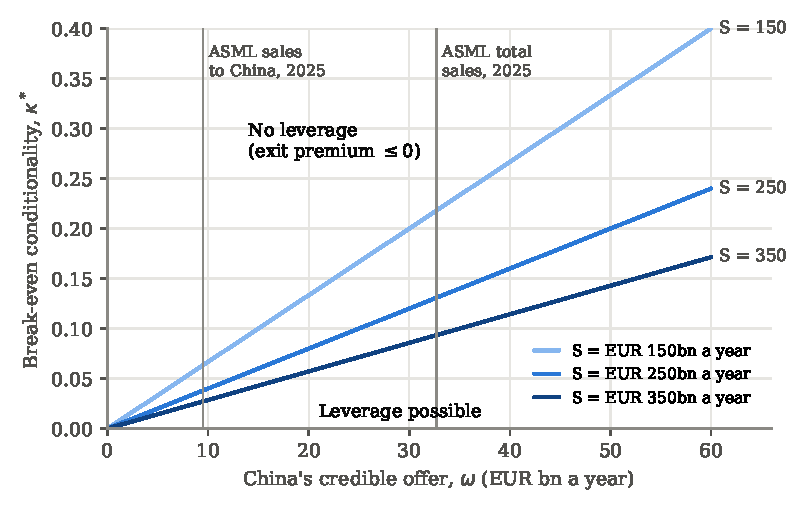
\includegraphics[width=0.78\textwidth]{figures/fig_breakeven.pdf}
\caption{Break-even conditionality of the US security guarantee. Lines show $\kappa^* = \omega/S$ for three values of the annual cost $S$ of replacing US protection. Above a line Europe's exit premium is negative and its leverage is zero. All other exit costs are set to zero, which favours Europe. Vertical rules mark ASML's 2025 sales to customers in China and its total 2025 sales \citep{asml2026annual}.}
\label{fig:breakeven}
\end{figure}

\subsection{The scenario}

\Cref{tab:scenario} summarizes what the model says about each episode.

\begin{table}[t]
\centering
\small
\caption{Europe 2031 through the model}\label{tab:scenario}
\begin{tabularx}{\textwidth}{@{}p{2.6cm}X p{2.2cm}@{}}
\toprule
Episode & What the model says & Result used\\
\midrule
2028: the Dutch halt DUV servicing in China & An equilibrium. The demand concerns hedging, so Washington uses jurisdiction over the hedged flows (the FDPR), not linkage. With high US jurisdictional reach and existential firm-level penalties, Europe's hedging premium is negative and it receives nothing. Solidarity from other member states does not change the reach of US jurisdiction. & \Cref{prop:main,prop:hedge}\\
2029: tiered AI access and the failed countermeasure & Rationing a loyal Europe removes the conditional part of the AI lever and raises Europe's exit premium. The countermeasure's failure does not follow: the named opponents hold 28.05 percent of EU population. Tier 1 status for the Netherlands alone is divide and rule. & \Cref{prop:statics}(b), \cref{prop:nested}\\
2031: the ultimatum & A preventive demand for control rights, issued as Europe's exit premium is expected to turn positive and made public to make the threat credible. The threat of permanent exclusion is not credible. China's threat to punish signing raises the bite Washington needs and the chance of breakdown. & \Cref{prop:control,prop:breakdown}, \cref{lem:selflimit}\\
2031: the US stockpile & Plausible for tools, much less so for servicing and parts. It matters only if the US buffer exceeds Europe's endurance horizon. & \Cref{prop:holdup}\\
Epilogue: compute on European soil & Raises Europe's buffer and makes AI denial costly for Washington (it lowers the US gain from denial), which weakens the conditional AI lever. & \Cref{lem:credible}(ii), \cref{prop:holdup}\\
Epilogue: a coalition of middle powers & Japan and Korea face the same structure. We conjecture that a coalition helps only if its assets are complements for the rival and its members can compensate one another; the model does not analyze coalitions of holders. & Conjecture\\
\bottomrule
\end{tabularx}
\end{table}

\paragraph{2028.} The scenario's first crisis is an equilibrium of the game it describes. The demand is to stop hedging, not to prevent exit, and \cref{prop:hedge} predicts that Washington will use flow-specific jurisdiction rather than the security or AI levers it needs to deter exit. That is what the scenario's Washington does when it threatens the FDPR. Because the penalty would be existential for the firm and the revenue at stake is a fraction of its sales, compliance follows even if the threat is partly a bluff. Europe gets nothing because its hedging premium is negative, not because it negotiated badly. The scenario's remedy for 2028, more solidarity among member states, would not have changed this: solidarity does not reduce US jurisdiction over a firm whose light source is made in San Diego.

\paragraph{2029.} The Frontier Inference Services Rule has an effect the scenario does not draw out. By cutting allocations to most of Europe while it remains aligned, Washington removes the conditional part of its AI lever. In the model this raises Europe's exit premium (\cref{prop:statics}b) and starts the drift that motivates the 2031 ultimatum. The failed countermeasure is harder to square with the model, because it is harder to square with the Council's voting rules. Under the 2026 population weights, the Netherlands, Ireland, Poland, the three Baltic states, and an abstaining Italy hold 28.05 percent of the EU's population, so twenty members with almost 72 percent remain in favour, more than the 55 percent of members and 65 percent of population that a qualified majority requires. For the measure to fail, a large state such as Germany, France, or Spain would have to defect as well, or the coalition would have to widen considerably, for instance to Romania, Czechia, and Hungary. Any thirteen members could also block. A US divide-and-rule strategy in the Council would therefore have to reach either a large state or a broad coalition of small ones.

\paragraph{2031.} The ultimatum is a preventive demand for control rights of the kind \cref{prop:control} characterizes. Europe is drifting: Chinese credit lines raise China's credible offer, five years of being treated as a vassal erode the value Europe places on a guarantee to the loyal, and rationing has removed the AI lever's conditional part. A forward-looking Washington acts while its threat still bites, and it goes public to make the threat credible. Two features of the scenario do not survive. The first is the threat that Europe will lose ``all access, present and future'' to American AI. \Cref{lem:selflimit} shows that a permanent cut hands Europe the exit option at the moment its future premium is positive, so the threat is credible only for a limited period. The second is the scenario's suggestion that China's counter-threat leaves Europe worse off whatever it does. China's threat is conditioned on signing with Washington. By \cref{prop:control,prop:breakdown}, a threat of that kind raises the bite Washington needs and the probability that the ultimatum is refused, which protects European ownership.

\subsection{The record, 2019--2026}

\paragraph{Compliance with in-kind payment.} The Dutch sequence from 2019 to 2025 is what \cref{prop:main} predicts for a holder in the region $Q\leq 0$: alignment without a cash transfer. What the Netherlands did receive fits the model's account of in-kind transfers. The December 2024 rule exempted countries with equivalent controls from the new foreign direct product rules \citep{bis2024fdpr}. That exemption costs Washington almost nothing, keeps the formal decision in The Hague, and can be withdrawn at will. It is a carrot made of the same jurisdiction that \cref{prop:statics}(c) identifies as Washington's cheapest stick.

\paragraph{Servicing and the MATCH Act.} By 2026 the live dispute was servicing of China's installed base, the hedge in our terms, and the instrument Washington reached for was flow-specific jurisdiction backed by legislation \citep{baumgartner2026match}, as \cref{prop:hedge} predicts. A statute also does something the model treats as an audience cost: it ties the hands of the executive and makes the threat harder to bargain away. The Dutch response was voice without exit. The prime minister raised the bill with the president and the trade minister lobbied Congress \citep{nltimes2026irritated}, but no one in The Hague suggested that the Netherlands might stop aligning. Two other features of 2026 also fit the model. Beijing's April 2026 regulations against foreign extraterritorial measures raised the firm's cost of complying with US servicing bans \citep{reedsmith2026decree}. Chinese customers pulled orders forward to stockpile tools, which is the wasting-asset problem in concrete form \citep{asml2026q3}.

\paragraph{Nexperia.} The Nexperia dispute shows China's coercive capacity at work and where its costs fell. China punished a Dutch move that followed a US rule by withholding chips from European carmakers, which spread the cost across member states. The Dutch government suspended its order, and relief came mainly through the US--China deal at Busan, in which Washington suspended its own affiliates rule \citep{taylorwessing2025nexperia, mofcom2025suspension}. In the terms of \cref{prop:statics}(d), China's coercion was a tax on the alliance, and the United States ended up paying it.

\paragraph{The guarantee.} The model's most direct implication for the transatlantic relationship concerns conditionality. Washington's 2025 strategy document links ``favorable treatment'' to export-control alignment \citep{whitehouse2025nss}, which raises conditionality. Troop withdrawals and open doubt about the commitment to loyal allies lower the value of the guarantee to the loyal, $\pi_A$, which lowers it. By May 2026 only 11 percent of respondents in a fifteen-country poll saw the United States as an ally \citep{ecfr2026home}. If Europeans come to believe that Washington will not defend them whatever they do, defence dependence stops buying Washington leverage over ASML. The Dutch trade minister's complaint about the MATCH Act is consistent with that change, though one episode cannot establish it.
